\section{Experiments}\label{sec:experiments}

We evaluated the real-world applicability of our approach while comparing the 2D image and 3D octree observations.

\subsection{Experimental Setup}\label{ssec:experimental-setup}

Throughout the experiments, we used a Summit XL-GEN mobile manipulator from Robotnik equipped with a 7~DOF Kinova Gen2 robotic arm and a three-finger mechanical gripper. The robot was controlled via MoveIt~2 both inside simulation for training and during sim-to-real evaluation in a Moon-analogue facility. To obtain visual observations inside the simulation, a virtual camera with a resolution of 128\(\times\)128~px was used at a framerate of 15~Hz. On the real robot, we used Intel RealSense D435 to capture images of 424\(\times\)240~px at 15~Hz, which were cropped and resized to 128\(\times\)128~px before use. We attached the camera statically at the front of the rover while randomizing its simulated pose during the training. To estimate the transformation between the real camera and the base of the real robot, we performed a hand-eye calibration. We did not employ any additional artificial lights mounted on the robot and relied solely on ambient illumination that originated either from the simulated Sun or a light source inside the Moon-analogue facility that emulates the solar illumination. For octrees, we used an observable volume of~40\(\times\)40\(\times\)40~cm in front of the rover, which results in the size of~2.5~cm for the finest leaf octants at the selected maximum depth of~\(d_{max}=4\). In order to avoid exploring areas of no interest, the position of the gripper was restricted to a~35\(\times\)35\(\times\)60~cm workspace centered at the origin of observable volume.

\subsection{Hyperparameters}\label{ssec:hyperparameters}

Because the selection of hyperparameters can significantly affect the learning curve and final performance of learned policies, we optimized hyperparameters in two consecutive steps. First, an automatic optimization was performed using the hyperparameter optimization framework Optuna~\cite{akiba_optuna_2019}. This was followed by subsequent fine-tuning of targeted hyperparameters via manual optimization. During this process, we also tuned the aforementioned reward scale, the number of observation stacks and the size of neural networks. The utilized set of hyperparameters can be seen in Table~\ref{tab:hyperaparameters}.

\begin{table}[ht]
	\centering
	\caption{Hyperparameters used for the training of all agents.}
	\label{tab:hyperaparameters}
	\vspace{-0.25\baselineskip}
	\begin{tabular}{lc}
		\hline
		\textbf{Hyperparameter}        & \textbf{TQC}                                \\ \hline
		Optimization algorithm         & Adam~\cite{kingma_adam_2014}                \\
		Learning rate schedule         & Linear, \(2.0 \cdot 10^{-4} \rightarrow 0\) \\
		Mini-batch size                & \(64\)                                      \\
		Gradient steps per update      & \(100\) (after every episode)               \\
		Size of the replay buffer      & \(50000\)                                   \\
		Discount factor \(\gamma\)     & \(0.99\)                                    \\
		Target update rate \(\tau\)    & \(4 \cdot 10^{-5}\)                         \\
		Entropy coefficient \(\alpha\) & Automatic~\cite{haarnoja_soft_2018}         \\
		Entropy target                 & \(-dim(\mathcal{A})=-5\)                    \\
		Number of critics              & \(2\)                                       \\
		Number of atoms                & \(25\)                                      \\
		Number of truncated atoms      & \(3\)                                       \\
		Exploratory action noise       & \(\mathcal{N}(0, 0.025)\)                   \\  \hline
	\end{tabular}
	\vspace{-0.8\baselineskip}
\end{table}

\subsection{Training Procedure}\label{ssec:training-procedure}

We trained agents in our simulation environment to learn policies for grasping lunar rocks by the use of TQC. In order to evaluate the proposed use of octree observations, we trained separate agents that use either image or octree observations. For image observations, we employed images with the resolution of 128\(\times\)128~px and two channels that contain the depth and intensity values for each pixel. Both of these values are normalized to be in the range~\([0,1]\), where the maximum distance of~1~m is selected for the depth map. Similar to octrees, two consecutive images are stacked together for each observation to preserve temporal information. To provide a fair comparison, an analogous feature extraction network architecture is created for image observations based on the octree-based feature extractor from Fig.~\ref{fig:actor-critic-network} by replacing 3D operations with their 2D variants. To achieve approximately the same number of learnable parameters for the feature extractor, i.e.~315k parameters, we increase the number of channels in 2D convolutional layers. The resulting network architecture for the image-based feature extractor is illustrated in Fig.~\ref{fig:image-feature-extractor}.

\begin{figure}[ht]
	\centering
	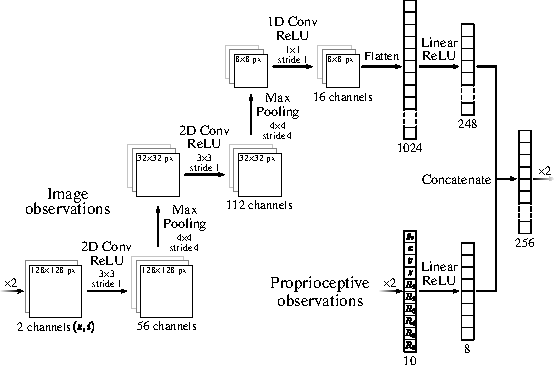
\includegraphics[width=1.0\linewidth]{image_feature_extractor.pdf}
	\caption{The network architecture of the image-based feature extractor, which is analogous to the octree-based feature extractor presented in Fig.~\ref{fig:actor-critic-network}.}
	\label{fig:image-feature-extractor}
\end{figure}

We also evaluated the importance of domain randomization for sim-to-real transfer in lunar applications. To do this, we trained agents on two different variants of the environment for each observation type. The first variant is the environment with complete domain randomization, whereas the second variant has a reduced level of randomization. In this reduced environment, only the pose of objects and the initial joint configuration are randomized for each episode. From the utilized datasets, one model of the lunar surface and four models of lunar rocks are randomly selected and used throughout the training. All other variables, such as the pose of the camera and the direction of illumination, are similarly selected at random but kept static throughout the training.

All agents were trained for 500k time steps and periodically evaluated every 10k steps on 20 episodes by utilizing their current policies with deterministic actions. For each analyzed variant, we trained three agents with different seeds for the pseudorandom generator that initializes the simulation environment and all learnable parameters. Since we evaluate the agents in a Moon-analogue facility located on Earth, the gravity of the simulated environment is set to~9.807~m/s\(^2\). Learning curves of all agents can be seen in Fig.~\ref{fig:results-learning-curve}.

\begin{figure}[ht]
	\centering
	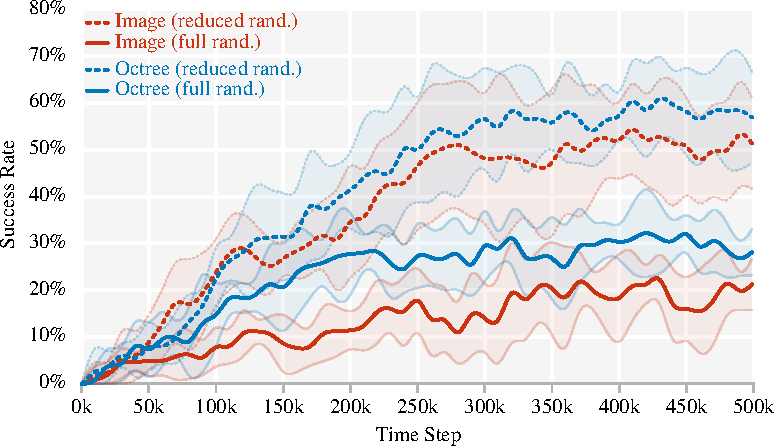
\includegraphics[width=1.0\linewidth]{learning_curve_plot.pdf}
	\caption{Learning curves of the trained agents that are evaluated every 10k steps. Solid lines represent smoothed mean, whereas shaded areas indicate the standard deviation over three runs with different random seeds.}
	\label{fig:results-learning-curve}
\end{figure}

\subsection{Sim-to-Real Transfer}\label{ssec:sim-to-real-transfer}

We evaluated the feasibility of sim-to-real transfer in LunaLab~\cite{ludivig_building_2020}, which is a Moon-analogue facility at the University of Luxembourg. We assessed all variants of trained agents, where the best performing agent at the end of its training inside the simulation is selected for each variant. The policies of these agents were then used for deterministic selection of actions during execution on the real robot. A~total of eight different rocks from Fig.~\ref{fig:test-rocks} were utilized during this experiment, where~1~--~4 rocks were randomly scattered within the workspace for each episode. Every agent was evaluated over the course of 25 episodes that were considered successful if the robot grasped and lifted one of the rocks.

\begin{figure}[ht]
	\centering
	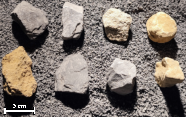
\includegraphics[width=0.8\linewidth]{test_rocks.pdf}
	\caption{Eight rocks used during the evaluation of the sim-to-real transfer.}
	\label{fig:test-rocks}
\end{figure}

Quantitative results of the sim-to-real success rate appear in Table~\ref{tab:sim_to_real_success_rate}, whereas an example of a successful grasp sequence is visualized in Fig.~\ref{fig:grasp-sequence}. During episodes that failed due to timeout, it was observed that agents got frequently stuck in a loop attempting to repeatedly grasp a specific rock without success due to improper positioning of the gripper. This behavior occurred for all evaluated agent variants, but it was most prominent for agents trained in environments with reduced domain randomization.

\begin{table}[ht]
	\vspace{1.379mm}
	\centering
	\caption{Quantitative results of the zero-shot sim-to-real transfer.}
	\label{tab:sim_to_real_success_rate}
	\vspace{-0.25\baselineskip}
	\begin{tabular}{ccc}
		\hline
		\textbf{Observation type} & \textbf{Level of randomization} & \textbf{Success rate} (n=25) \\ \hline
		Image                     & Reduced                         & 12\%                         \\
		Image                     & Full                            & 20\%                         \\
		Octree                    & Reduced                         & {\phantom{0}}8\%             \\
		Octree                    & Full                            & 32\%                         \\ \hline
	\end{tabular}
	\vspace{-0.8\baselineskip}
\end{table}

\begin{figure}[ht]
	\centering
	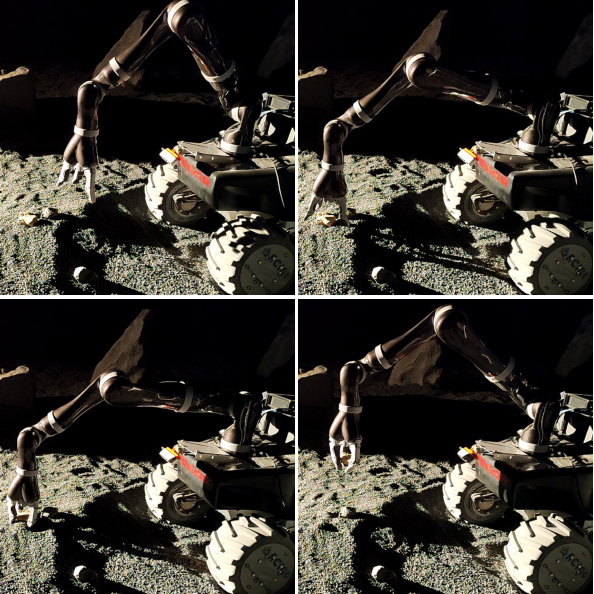
\includegraphics[width=1.0\linewidth]{grasp_sequence.pdf}
	\caption{An example of a successful grasp sequence using the real robot.}
	\label{fig:grasp-sequence}
	\vspace{-1.0\baselineskip}
\end{figure}
